% !TEX root = ../main.tex

% 中英标题:\chapter{中文标题}[英文标题]
\chapter{带自交的遗传算法设计与实现}[Model Solving Scheme Based on Improved Genetic Algorithm]

\section{经典遗传算法的改进}[Improved algorithms]
与经典的遗传算法相比,本文提出的算法有以下改进点:
% \begin{itemize}
%	\item [(1)] 在算法中加入多轮筛选,对不符合无人机载重要求的个体予以删除,符合优质个体多繁衍,劣质个体少繁衍甚至不繁衍的自然选择规律;
%	\item [(2)] 类似孟德尔豌豆杂交实验,在适应度计算完成后对优秀的个体进行自花授粉,以保留优秀个体的基因;
%	\item [(3)] 对轮盘赌选择方法进行了改进,避免削弱种群的规模和降低种群多样性,防止陷入局部最优解;
% 	\item [(4)] 对交叉过程进行了改进,尽量避免了交叉过程后存在有无人机在运输过程中超重的问题。
% \end{itemize}
\begin{itemize}
	\item [(1)] 在种群初始化、交叉操作和变异操作后加入了对个体的筛选过程。由于无人机载重有限,存在最大载重值,如果有无人机的线路规划中存在无人机超重运输的情况,这类个体应该被淘汰掉,而不是继续繁衍从而挤压其余个体的生存空间。因此本文在这三个过程后加入了筛选过程,对不符合无人机载重要求的个体予以淘汰,
从而使得算法更加符合“优质个体多繁衍,劣质个体少繁衍甚至不繁衍”的自然规律;
	\item [(2)] 类似孟德尔豌豆杂交实验,模拟了人工培养豌豆授粉的过程,在适应度计算工作完成之后,让优秀的个体进行自花授粉,将劣势的个体进行淘汰。选出适应度较高的个体进行自交,跳过选择过程,而是直接进入变异过程,这样可以减少选择、交叉过程中对优秀基因可能存在的破坏,让优势个体
更加顺利地进入下一代的繁衍过程;
	\item [(3)] 经典的遗传算法中采用的轮盘赌算法是很经典的选择方法,其基本思想是个体被选择的概率与个体的适应度函数的值成正比,这样可以防止适应度函数值较小的个体被直接淘汰,但是这种方法也存在被选择概率高的个体被多次选中,从而削弱种群规模,降低种群的多样性的问题,从而有可能使问题的解陷入局部最优解的情况。
因此改进后的遗传算针对轮盘赌算法也进行了一些改进;
	\item [(4)] 由于改进后的遗传算法在流程中加入了多轮筛选,在染色体交叉过程中很可能会产生较多会使无人机超载的路径规划,因此算法改进了交叉过程的交叉方式,尽量避免了存在超载问题。
\end{itemize}


由于改进后算法的流程与经典遗传算法的主要区别是加入了类似孟德尔豌豆杂交实验中的自交过程,因此该算法被称为带自交的遗传算法(Genetic Algorithm With Selfing, GAWS)。
\section{带自交的遗传算法的描述}[Algorithm design]

\subsection{染色体的编码方法}[Method of chromosome coding]
在遗传算法中,染色体的编码方法主要有二进制编码法、符号编码法和自然数编码法等。在本问题中,具体选择的是自然数编码法。


自然数编码由自然数$1,2,\cdots,n$组成,这些基因位代表的是兴趣点,而基因的序列则代表无人机对兴趣点的访问顺序。$0$在编码中表示的是基地$B$,由于无人机从基地$B$出发,
完成配送任务后又返回基地$B$,因此单架无人机的访问顺序总是从$0$开始,而又从$0$结束。基地$B$的编码$0$又可以很方便地将不同无人机的线路分离。自然数编码能够很好地反映
无人机参与救援的过程,便于后面代码的撰写,因此选择了该编码方法。


在本问题中,基地$B$中停放有$m$架无人机,对$n$个兴趣点实施救援。由于在整个流程中,每个兴趣点只被访问一次,所以无人机的数量决定了子路径的数量,从而本问题中一条染色体的长度
为$m+n+1$。例如,一条染色体的编码为``0 7 8 0 4 5 6 0 1 3 2 0 9 0'',这代表$4$架无人机同时对$9$个兴趣点进行救援,所有的子路径为:
$$0\rightarrow7\rightarrow8\rightarrow0,0\rightarrow4\rightarrow5\rightarrow6\rightarrow0,0\rightarrow1\rightarrow3\rightarrow2\rightarrow0,0\rightarrow9\rightarrow0$$

\subsection{种群的初始化设计}[Population initialization design]
初始化种群时,本文采用随机访问的方法进行设计。首先随机产生一条无人机的配送子路径,如果无人机根据这条路径运送救援物资能够不超出无人机的最大载重$w$,则存储这条路径,反之抛弃这条路径,
然后重复这个过程,直到所有的兴趣点都被无人机访问。


将以上的子路径组合起来,并将基地$B$用自然数$0$进行表示,连接这些子路径,可以得到一条包含所有兴趣点的染色体,这个染色体就是一套完整的无人机调度方案。在本问题中,将初始种群个数设置为
$100$,即在初始化过程中会产生$100$条符合要求的染色体。

\subsection{适应度函数设计}[Design of fitness function]
使用自然数对染色体进行编码,可以保证无人机的飞行路径较为清晰,但是不能确保在进化过程中产生的新路径能够一定满足不超重和尽可能少超时,所以为了确保进化过程中能产生最优解,本文需要引入一个惩罚函数,
对不合理的路径规划结果进行惩罚:
\begin{equation}
	f= \alpha d_s + \beta m_s + \gamma w_s
\end{equation}

其中,$d_s$是无人机的飞行距离之和,$m_s$是所有子路径中无人机的超重数量之和,$w_s$是所有子路径中无人机超出时间窗之和。而$\alpha,\beta,\gamma$是系数,根据各参数的重要性,将这些参数设置为
$\alpha = 1,\beta = 10,\gamma = 100$。


由于各参数的单位不统一,在计算惩罚函数时还需要对数据进行归一处理。


所有子路径中无人机超出时间窗之和$w_s$用以下公式表示:
\begin{equation}
w_s = \sum_{i=1}^n max\left\{\Delta t_i,0\right\}
\end{equation}

其中,$\Delta t_i$代表无人机从起飞到访问兴趣点$p_i$所花费的时间与该兴趣点的时间窗$ts_i$之差。


为了衡量个体的适应度,将适应度函数$F$设置为惩罚函数$f$的倒数:
\begin{equation} 
	F = \frac{1}{f}
\end{equation}

\subsection{择优过程}[Individual preference]
为了更好地模拟孟德尔豌豆实验,在算法中加入了对优秀个体自花授粉的过程。将初始化种群中的100个个体按照适应度大小进行排序,选择其前
$5\%$的的染色体进行自交,而其余的染色体则进入选择阶段。在自交过程中,会产生2倍数量的个体,他们跳过选择阶段和交叉阶段,直接进入变异过程,这样可以有效
保护优秀基因。

\subsection{选择过程}[selection process]
采用轮盘赌算法进行个体的选择。轮盘赌算法是一种回放式的随机采样方法,个体进入下一代的概率就是其适应度与整个种群个体适应度之和的比值,适应度的值越大,个体被选中的概率也就越大。
但是,传统轮盘赌算法误差较大,部分个体容易被多次选出,可能会削弱种群的规模和降低种群多样性,导致最终陷入局部最优解。为了避免这种情况,本文对轮盘赌算法进行了一些改进:
\begin{equation} 
	F_i' = F_i - F_{min} 
\end{equation}


其中,$F_i$是第$i$个个体的适应度,$F_{min}$是所有个体中适应度的最小值,其计算方法如下:
\begin{equation}
	F_{min} = min\left\{F\right\} 
\end{equation}


最后,可以计算出第$i$条染色体被选择的概率为:
\begin{equation}
	P(i) = \frac{F_i}{\sum F_i'} 
\end{equation}

\subsection{交叉操作}[Crossover operation]
在遗传算法中,交叉操作是指满足交叉概率$p_c$两个相互配对的染色体交换部分基因,形成新的个体。常用的交叉方式有单点交叉、两点交叉、多点交叉和均匀交叉等。由于该问题的特殊性,所有存在无人机超重情况的规划路径都
应该被剔除,因此这里在进行交叉操作时,需要使得结果尽量避免存在有无人机在运输过程中超重,交叉过程如\figref{fg401}所示:
\begin{figure}[ht]
	\centering
	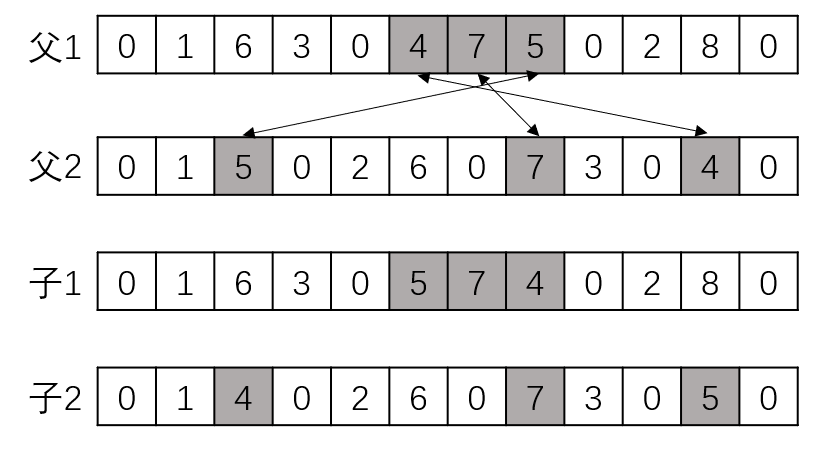
\includegraphics[width = 0.7\textwidth]{fg3_jiaocha}
	\caption{交叉操作过程示例}
	\label{fg401}
\end{figure}


\begin{itemize}
	\item [(1)] 针对满足交叉概率$p_c$的父代个体1和父代个体2,从父代个体1中随机选择一个子路径作为交叉片段(不包括子路径中的自然数0);
	\item [(2)] 从父代个体2中寻找与上述子路径编号对应的片段,作为父代个体2的交叉片段;
	\item [(3)] 交换父代个体1和父代个体2的交叉片段,得到子代个体1和子代个体2;
 	\item [(4)] 重复上述步骤,直到生成子代的数量符合要求。
\end{itemize}

\subsection{变异操作}[Mutation operation]
针对满足变异概率$p_m$的染色体,在兴趣点编号范围内随机选出两个不相同且不为0的数字,将染色体对应的基因编码进行交换,即为变异过程。变异过程如\figref{fg402}所示。
\begin{figure}[ht]
	\centering
	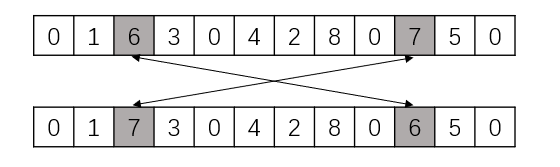
\includegraphics[width = 0.7\textwidth]{fg4_bianyi}
	\caption{变异操作过程示例}
	\label{fg402}
\end{figure}
\subsection{对基因的多轮筛选}[Multiple rounds of gene screening]
在种群初始化、交叉算子和变异算子后,选择对各条路径的载重约束进行检查。如果发现有个体对应的路径存在无人机超重配送的情况,应该对染色体予以删除,以符合无人机的飞行安全要求。


完成初次迭代后,算法会重复完成上述择优过程、选择过程、交叉操作和变异操作,以及对基因的多轮筛选,直至迭代次数符合初始设置时,算法结束。


带自交的遗传算法其伪代码如下:


\begin{algorithm}[H]  %其中这里面不能有H不然会报错,不过不影响结果
	\caption{带自交的遗传算法}%算法名字
	\LinesNumbered %要求显示行号
	\KwIn{兴趣点的集合$P$,兴趣点对应时间敏感性的集合$T_s$,兴趣点对应的救援物质需求的集合$S$,无人机的集合$U$,基地$B$,无人机的最大续航时间$T_{max}$,无人机的飞行速度$v$,最大载重$w$。}%输入参数
	\KwOut{无人机的飞行路径规划$O$,无人机的准时覆盖率$R_o$和有效覆盖率$R_e$}%输出
	检查$T_s$的值是否符合要求\; %\;用于换行
	$generations = 50~$//设置迭代次数为50\;
	$generation = 0~$//用于记录迭代次数\;
	PopInit()//对种群进行初始化\;
	Filter()//对种群进行筛选\;
	\While{$generation \le generations$}{
		FitnessCal()//计算适应度函数\;
		\eIf{个体适应度位于前5\%}{
			Selfing()//自交过程\;
		}{
			Select()//选择过程\;
			Cross()//交叉过程\;
			Filter()//对种群进行筛选\;
		}
		\If{满足变异概率}{
			Mutation()//变异过程\;
			Filter()//对种群进行筛选\;
		}
		$generations++$\;
	}
	计算无人机的准时覆盖率$R_o$和有效覆盖率$R_e$\;
	return $O,R_o,R_e$
	
\end{algorithm}


带自交的遗传算法其流程图如\figref{fg403}所示:
\begin{figure}[H]
	\centering
	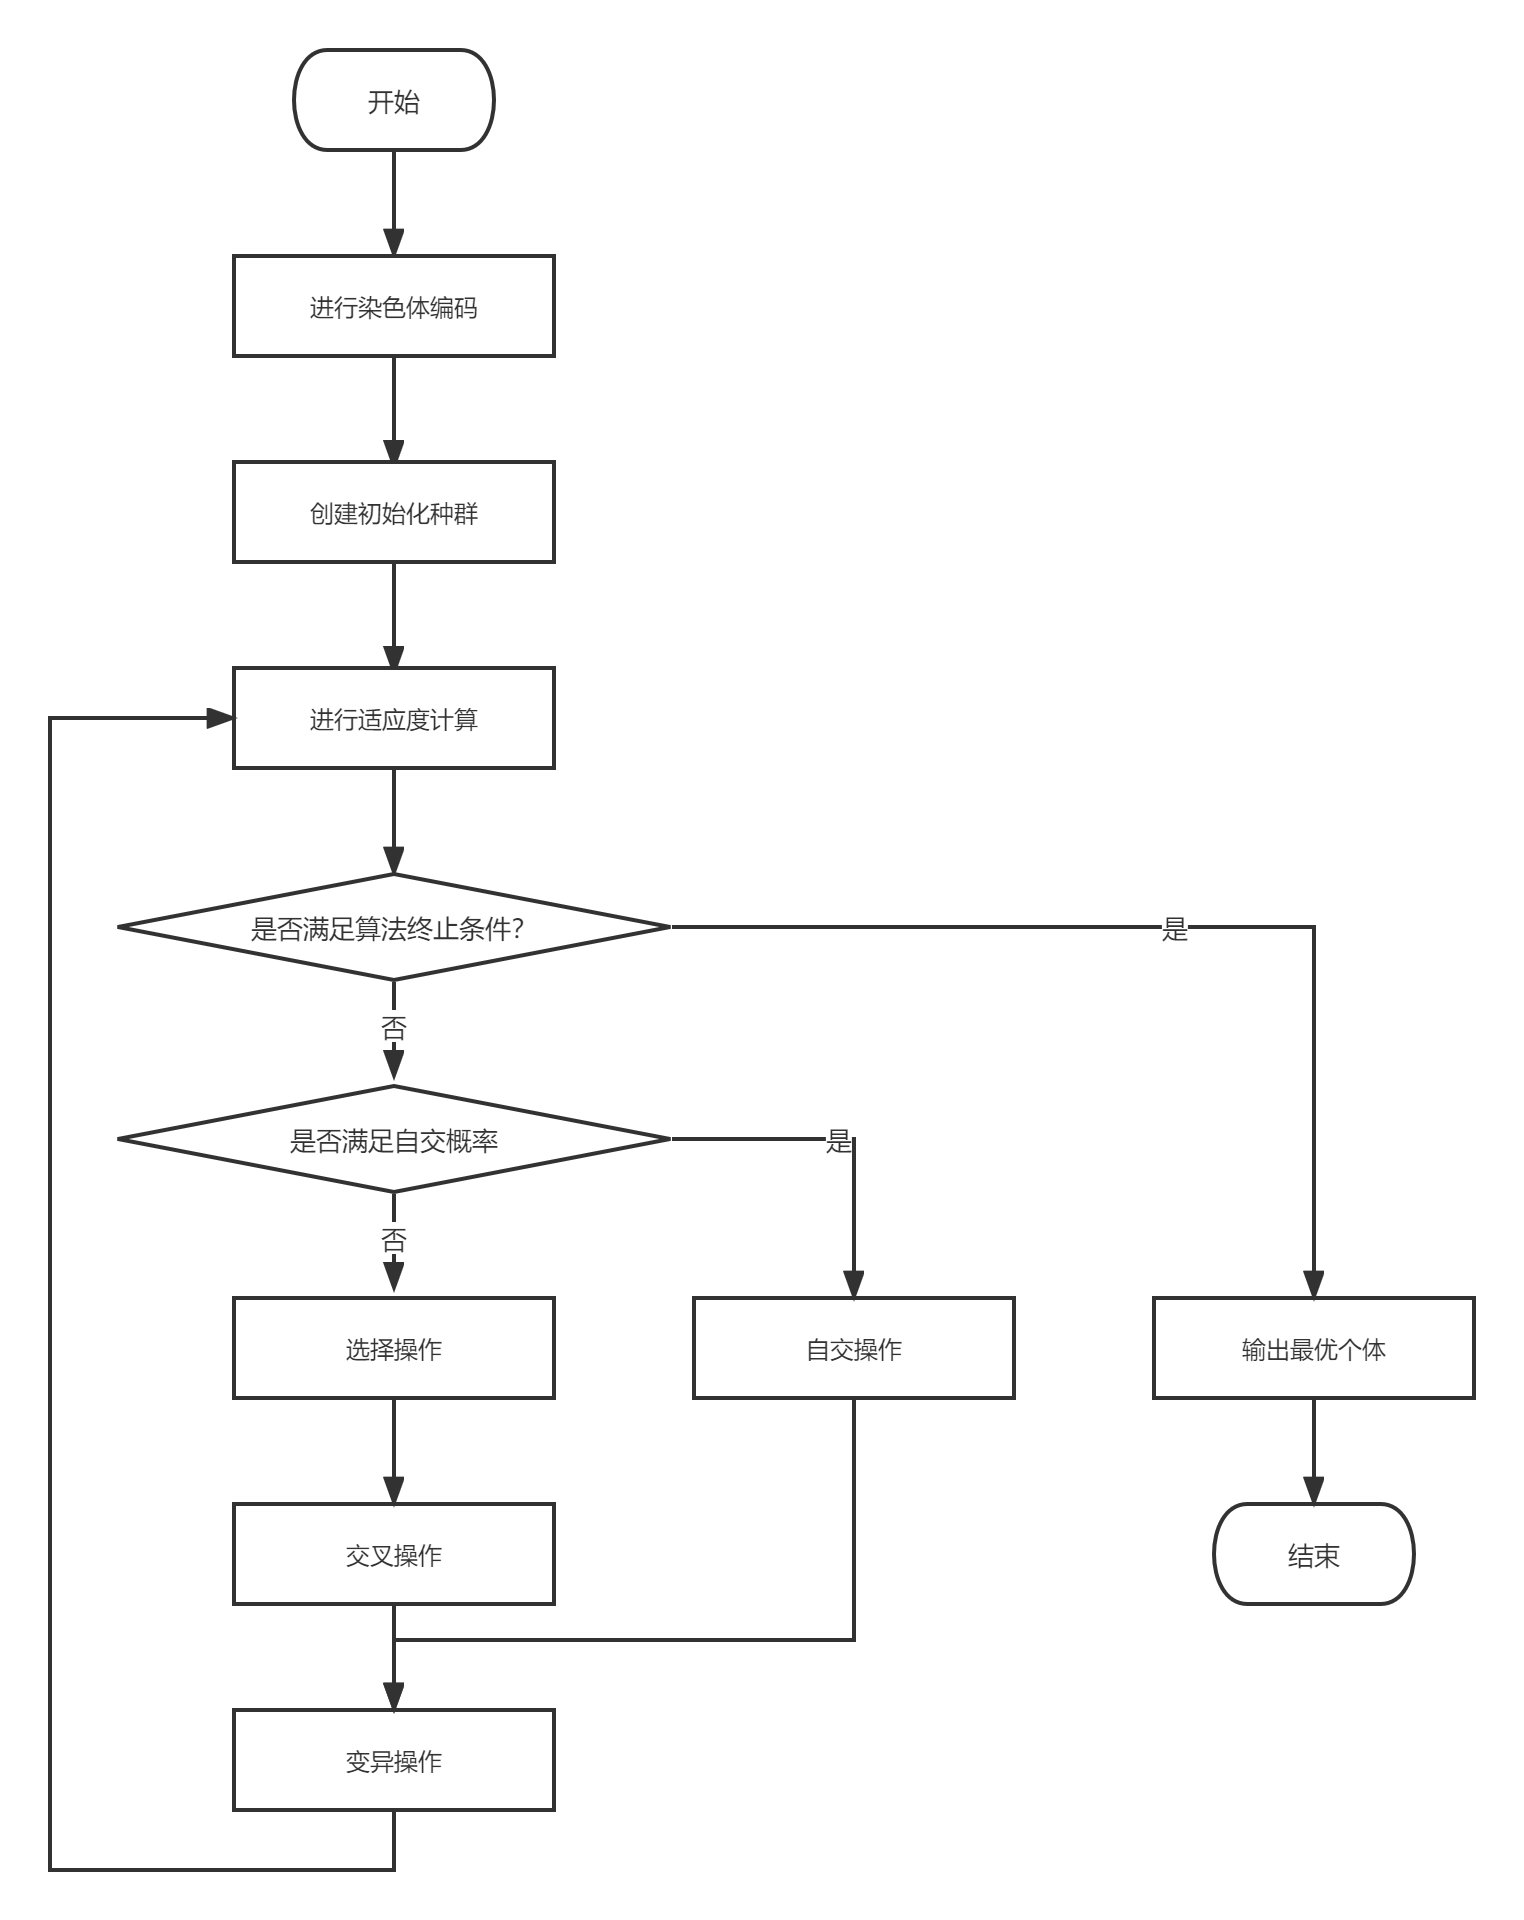
\includegraphics[width = 1.0\textwidth]{fg6_ga}
	\caption{带自交的遗传算法流程图}
	\label{fg403}
\end{figure}

\section{本章小结}[Brief summary]
本章主要对遗传算法的基本流程进行了介绍,并且针对经典遗传算法不足之处进行了一些改进,提出了带自交的遗传算法以解决带时间敏感的无人机扫描覆盖问题,该算法求解结果中无人机的有效覆盖率$R_e$相较经典遗传算法更高,且能降低无人机的飞行成本。